\documentclass{article}

\usepackage{graphicx}

\begin{document}

\begin{titlepage}
\title{Searching for circuit complexity lower bounds using SAT solvers}
\author{Candidate 1042155\\Trinity Term 2022\\MCompsci Computer Science}
\maketitle
\end{titlepage}

\begin{abstract}
Where the abstract will go
\end{abstract},

\tableofcontents

\section{Introduction}

\subsection{Motivation}

A Boolean circuit consists of a network of gates computing simple boolean functions such as AND, OR and NOT, connected such that on any input, the gates compute some set of outputs. Finding lower bounds on the size of circuits computing given Boolean functions is one of the most fundamental and most challenging problems in computer science. Results in this area can be used to separate computational complexity classes.

For example, since P (the class of problems decidable in polynomial time in the length of the input) is contained within $P_{/poly}$ (the class of problems decidable by a family of circuits each of whose size is polynomial in the length of the input), then to separate P from NP (problems decidable by a non-deterministic Turing machine in polynomial time) it suffices to prove that NP $\notin P_{/poly}$, i.e. to find a function in NP which cannot be decided by a polynomial-size family of circuits. This would prove that a large class of fundamental and practically useful problems do not necessarily have polynomially fast algorithms~\cite{arora}. 

The majority of functions do require exponential circuits, which can be seen from a simple counting argument noting that the number of possible circuits is far higher than the number of possible Boolean encodings of small circuits~\cite{arora}. Despite this fact, the best lower bounds proven on unrestricted circuits are only linear~\cite{boppana} and we still do not have optimal circuits or close upper and lower bounds for many important functions.

If functions with circuits of a given complexity could be identified by an efficient algorithm, this could be used to construct efficient learning algorithms for circuits of a smaller complexity; this would resolve one of the biggest questions in learning theory~\cite{carmosino}. Furthermore, such an algorithm could be used to break pseudorandom generators (i.e. distinguish random from pseudorandom inputs)~\cite{razborov94}. As a result, this problem has strong connections in both learning theory and cryptography. Proving circuit lower bounds would also imply derandomisation - that all randomised algorithms have a deterministic counterpart which is only polynomially slower~\cite{arora}.

A heuristic approach is to find minimal circuits for small instances of the functions. This can be used to prove new bounds~\cite{kulikovsurvey} and may lead to theoretical insights on the structure of their optimal circuits generally~\cite{williams}. Doing this for small functions computing natural functions like parity, modulo and addition allows us to gain a greater understanding of their difficulty and compute them more efficiently when using low-level code or hardware. 

Finding efficient circuits is also necessary in practice when designing electronic systems. Electronic circuit design is an extensive field of its own, involving circuit simulation software to test designs, or hardware specification languages such as Verilog and circuit synthesis software to convert specifications into circuits. However, electronic circuit design is concerned with a wider range of problems (for example, analogue and time-dependent functions) and with concerns about correct physical implementation; we focus on abstract circuits.

One approach to automating the search for efficient circuits is to reduce the problem of designing a correct circuit (logical design synthesis) to the Boolean satisfiability problem (SAT). Existing algorithms (SAT solvers) can then be used to solve the problem, either finding a correct circuit of fixed size or generating a proof that none exists~\cite{kulikov}. SAT solvers have become increasingly powerful in recent years and now have many industrial applications\cite{prasad}; the wide range of heuristics implemented by different SAT solvers means that one suited to the problem at hand could be found or developed. 

\subsection{Previous work}

Circuits are a popular model of computation; they are non-uniform, meaning that in a family of circuits where each takes a different size of input, each circuit is independent and not constructed by a common algorithm. Notably, this means that circuits are not subject to the Space and Time Hierachy Theorems, although there is a Non-Uniform Hierarchy Theorem stating that larger circuits can compute strictly more functions than smaller ones~\cite{arora}. In the past there have been theoretical proofs of lower bounds for restricted circuit classes, such as $AC^0$ (functions computed by circuit families of $O(1)$ depth)~\cite{furst81}~\cite{ajtai83}, $AC^0[k]$ (i.e. $AC^0$ additionally with MOD-k gates)~\cite{razborov87}~\cite{smolensky87}, and monotone circuits~\cite{razborov85}. There was also a bound showing the practical impossibility of deciding bounded-size formulae in a certain second-order language~\cite{stockmeyer02}. However, no lower bounds better than $(3+1/86)n-o(n)$ have been found for general circuits over the basis $B_2$ consisting of all functions on 2 bits~\cite{find16}, while the best bound is 5n-c for the basis $U_2 = \{ \land, \lor, \neg\}$~\cite{lachish01}~\cite{iwama02}. Furthermore, there are results stating that it is impossible to prove circuit lower bounds separating P and NP by relativising methods~\cite{baker75}, algebrizing methods~\cite{aaronson09}, or (under standard cryptographic assumptions of the existence of strong one-way functions) so-called `natural proofs'~\cite{razborov94}. A formula in Disjunctive Normal Form (DNF) is one consisting of clauses (disjunctions of literals), with the final formula consisting of the conjunction of all clauses; a $k$-DNF is one where the number of literals in one clause is at most $k$. It has been proved that circuit lower bounds are hard to prove using Resolution and Resolution with $k$-DNFS, and it is conjectured that they are also hard for stronger proof systems such as Frege systems~\cite{raz}. 

Due to this difficulty in theoretical progress, we would like to investigate the problem empirically. SAT solvers provide a useful heuristic, as they allow us to examine small examples of the problem and find concrete rather than asymptotic bounds; due to improvements in SAT solver performance over the past years, this approach has now been put into practice. For example, Kamath et al~\cite{kamath} propose a reduction from logical design synthesis to SAT which fixes the DNF structure of the circuit and number of disjunctions used. Experiments using this reduction to find minimal circuits for 2-4 bit adders and multipliers are reported in~\cite{estrada}. 

Kojevnikov et al~\cite{kulikov} demonstrate a more general reduction allowing any circuit with a fixed number of gates, using it to prove both upper and lower bounds for both specific functions and the general case. In particular, they prove linear bounds for \(MOD^n_3\) circuits (computing whether the number of bits is equal to n modulo 3) over different Boolean bases. This was done by checking for circuit `building blocks' with 5 to 11 gates. This was the first large-scale, direct attempt to use SAT solvers to search for circuit bounds.

In~\cite{kulikovlocal} Kulikov et al used the same reduction to improve large circuit building blocks by searching for smaller versions of their sub-circuits. Specifically, linear upper bounds were proved or verified for the symmetric functions \(SUM\), \(MOD^n_4\), and \(MOD^n_3\) by checking for circuits with up to 13 gates (they remarked that checking for existence of a Boolean circuit of size 13 was out of reach). They also improved on the best known lower bound for the threshold function (which outputs true if more than k input bits are set to true, for some k). Their technique allowed them to search for improvements on circuits that were much larger than a SAT solver could deal with if taken as a whole.

Knuth also used SAT solvers to investigate lower bounds for \(MOD^n_3\)~\cite{knuth15} (solution to exercise 480). Define $MOD^{m,r}_n(x_1 \ldots x_n) = [x_1 + \ldots + x_n \equiv r \ $mod$ \ m]$, where $[b]$ is the Iverson bracket, i.e. evaluates to 1 if $b$ evaluates to true, else 0.

Based on the minimum circuit sizes he found for small sizes of n, Knuth conjectured that for all $r$, and $n \geq 3$,

\[
  size(MOD^{m,r}_n) = 3n - 5 - [(n+r) \equiv 0 \ mod \ 3]  
\]

where $size(f)$ is the size of a minimal circuit over the $B_2$ basis which computes $f$. He was able to confirm this for $3 \leq n \leq 5$ and all $r$, and for the case $n=6, r=0$, but not for the case $n=6, r=1$.

\subsection{Our contributions}

We investigate feasible ways to find small circuits using SAT reductions. Previous research in this area has focused on a small number of target Boolean functions and a single reduction at a time. Instead, we use multiple combinations of reductions and SAT solvers to see which leads to the best performance, displayed in Section \ref{satresults}. In Section \ref{funcresults}, we tested them on a range of symmetric functions whose lower bounds are already somewhat understood, in order to analyse the performance in relation to the bound. 

We also search for a general relationship between solver performance and minimum circuit size in Section \ref{randomresults} by applying our methods to a sample of randomly generated functions. In Section \ref{knuthresults} we then use solvers to prove a result, that a lower bound conjecture about MOD-3 functions due to Knuth~\cite{knuth15} does not hold for the de Morgan basis $U_2$. 

From these experiments we note that available solvers running on a personal computer can decide the existence of some circuits of size 11 in just a few hours, while others of size 11 and 12 can take many hours on a high-powered computing cluster (13 and above were not investigated). That is to say, the amount of time taken to solve comparable problems can vary considerably.

Exploring an additional possibility for improving performance, we find that adding extension axioms to a problem can improve the performance of a SAT solver on it, even when they are chosen at random. However, this effect varies between different target functions, even when searching for circuits of the same size.

\section{Background}

\subsection{General setting}

Denote by \(B_{n,m}\) the set of all Boolean functions \(f: \{0,1\}^n \to \{0,1\}^m\) and let \(B_n = B_{n,1}\). A circuit over the basis \(A \subseteq B_2\) is a finite directed acyclic graph with nodes of in-degree 0 or 2. Nodes of in-degree 0 are called inputs. Nodes of in-degree 2 are assigned functions from \(A\) and are called gates. Some nodes may be also be marked as outputs.

Without loss of generality, we can also assert that every gate has a larger index than both of its predecessors (i.e. the gates are sorted topologically w.r.t. the used numbering); that every gate's second predecessor has a larger index than its first predecessor; and that the last gate is an output ~\cite{kulikov}.

A circuit \(C\) of size $N$ is said to compute the function \(f\in B_{n,m}\) if, for all input vectors \(v\in\{0,1\}^n\) in the range of \(f\), \(C(v)=f(v)\), where \(C(v) = (o_1,...o_m)\) are the values of the output gates of \(C\), each input \(x_i\) takes value \(v_i\), and each gate takes the value of its assigned function when applied to the value of its two predecessor nodes.

In this paper, we mainly consider circuits over the De Morgan basis \[U_2 = \{\lor, \land, \neg\}\] where \(\neg\) denotes the Boolean function which outputs the negation of its first argument.

The size of a circuit is its number of gates. We define the Minimum Circuit Size Problem (MCSP) as the question of whether, given a natural number $N$ and a function \(f: \{0,1\}^n \to \{0,1\}^m\), there exists a circuit of size $N$ computing \(f\).

\subsection{SAT solvers}

SAT solvers have previously seen success in proving mathematical theorems, most famously in 2016 when Heule et al solved the Boolean Pythagorean Triples problem~\cite{heule} and in 2020 when Brakensiek, Heule et al solved Keller's conjecture~\cite{heule2}. In general, SAT solvers have the advantage of being effective even when heuristics are not known for solving the original problem, as in our case of MCSP.

Modern SAT solvers are based on conflict-driven clause learning (CDCL). This is an algorithm closely related to the Davis–Putnam–Logemann–Loveland (DPLL) algorithm, and which is also based on the Resolution proof system~\cite{cdcl}~\cite{krajicek}. The general idea of DPLL is to choose an assignment to a variable, propagate it (simplify the problem by removing clauses that now evaluate to true), and repeat until either finding a satisfying assignment, or finding that our assignment makes the formula unsatisfiable: in which case `backtrack' (remove the last assignment until the formula is no longer unsatisfiable - if this is impossible, the answer is UNSAT) before trying again with a different assignment. This is essentially a form of depth-first tree exploration. The major difference in CDCL is that it adds a `learned clause' to the formula when it reaches an unsatisfiable assignment, according to a procedure incorporating Resolution; it backtracks until the learned clause is also satisfiable, allowing it to avoid some other unsatisfiable assignments~\cite{bayardo97}.

For this project we used 4 different SAT solvers, all based on CDCL. As mentioned earlier, this means that they cannot decide general circuit lower bounds with a less than exponential-length proof~\cite{raz}. However, this is an asymptotic bound and still allows for reasonably-sized proofs for small inputs such as the ones investigated in this paper. 

MiniSAT~\cite{minisat} was the winner of the 2005 SAT Competition and was last updated to version 2.2 in 2010~\cite{minisat2010}. Despite being old, it is well-documented and the other solvers we used were based on it, making it a good baseline for performance. It was also one of the solvers used to decide MCSP in~\cite{kulikov}.

PicoSAT is a solver inspired by miniSAT 1.14, with a focus on improving low-level performance by using optimised data structures~\cite{picosat}. It was submitted in the 2010 SAT-Race, and was also one of the solvers used in~\cite{kulikov} and the main one in~\cite{kulikovlocal}, which is why it was chosen.

MapleSAT is the most recent solver, chosen for its good track record, with variants having won the SAT Competition 2016 and placed second in 2017. It was based off MiniSAT 2.2 but has a different branching heuristic, incorporating ideas from machine learning\cite{maplesat}.

Finally, in order to make full use of the Oxford ARC service and its distributed computing, the parallel solver Glucose-Syrup was used. This is a 2014 parallel version of the Glucose solver which placed 4th in both the 2014 and 2015 SAT Competition. Glucose is a solver also based on MiniSAT 2.2, which uses a new heuristic to more accurately estimate the `usefulness' of its learned clauses and regularly delete ones that are not as useful~\cite{glucose}. Glucose-Syrup is an unusual `non-portfolio' parallel solver which runs multiple instances of the same solver in parallel, but rather than taking a divide and conquer approach, uses new heuristics for sharing learned clauses between the instances in order to speed them up~\cite{glucose-syrup}.

These open-source SAT solvers take input in the form of text files in the DIMACS format~\cite{dimacs} and need to be run from the command line; for this project, we wrote a TypeScript library to store CNF formulae together with comments and output them correctly both in human-readable and DIMACS formats.

\subsection{Extension axioms}

A relatively unexplored method for speeding up SAT solvers is adding extension axioms to the initial formula by the following method:

\begin{enumerate}
  \item Let $l_1$, $l_2$ be existing literals chosen from the formula and let $q$ be a fresh variable, known as the extension variable.
  \item Add the clauses
  \[
    \{\neg l_1, q\}, \{\neg l_2, q\}, \{l_1, l_2, \neg q\}
  \]
  These are known as extension axioms.
  \item Repeat arbitrarily many times with new choices for $l_1$, $l_2$ and new fresh variable $q$. Note that the previously added $q$ may also be chosen as a literal.
\end{enumerate}

These axioms allow the SAT solver to use `Extended Resolution' - resolving on a formula incorporating multiple literals, rather than on a single literal. This is possible since $q \leftrightarrow l_1 \lr l_2$ and $l_1$, $l_2$ may also be extension variables, allowing for larger formulae to be built~\cite{krajicek}. Some statements that require an exponential length proof in Resolution require only a polynomially long proof in Extended Resolution, e.g. a formula stating the pigeonhole principle~\cite{cook79}.

\subsection{Reduction to SAT}

We encoded the MCSP as a Boolean formula using three reductions. Let $t$ be the target function with $n$ inputs, and let $N$ be the number of gates required in the circuit.

\subsubsection{Kojevnikov reduction}

The first is due to Kojevnikov et al~\cite{kulikov} who present it together with bounds on the growth rate of the formula. In particular, the growth rate of the number of clauses is $O(N \cdot 2^n)$. The basis of the circuit can be restricted to any subset of \(B_2\).

It uses the following variables:

\begin{enumerate}

  \item $t_{ib_1b_2}$ $(n \leq i < n + N, 0 \leq b_1 < 2, 0 \leq b_2 < 2)$ is the value of the $i$-th gate if its first predecessor takes value $b_1$ and its second takes value $b_2$. The four variables $t_{i00}, t_{i01}, t_{i10}, t_{i11}$ thus define the function assigned to the $i$-th gate. This gives $O(N)$ variables.
  \item $c_{ikj}$ $(n \leq i < n + N - 1, 0 \leq k < 2, 0 \leq j < n + N)$ is true iff $j$ is the $k$-th predecessor of $i$. This gives $O(N^2)$ variables.
  \item $o_{ij}$ $(n \leq i < n + N, 0 \leq j < m)$ is true iff the $j$-th output is computed by the $i$-th gate. This gives $O(Nm)$ variables.
  \item $v_{it}$ $(0 \leq i \leq n + N, 0 \leq t < 2^n)$ is the output value of the $i$-th gate if the input variables take values represented by the bits of $t$. These are used to constrain correctness of the circuit on all possible inputs, including its outputs matching the truth table of the encoded function.

\end{enumerate}

We encode the requirements for the circuit by the following clauses:

\begin{enumerate}

  \item The binary function assigned to each gate belongs to our desired basis.
  \item For all $(i,k)$, exactly one variable $c_{ikj}$ is true (there is exactly one $k$-th predecessor of the $i$-th gate). This gives $O(N^3)$ 2-clauses and $O(N)$ $O(N)$-clauses.
  \item For all $j$, exactly one variable $o_{ij}$ is true (the $j$-th output is computed by exactly one gate). This gives $O(N^2m)$ 2-clauses and $O(m)$ $O(N)$-clauses.
  \item For all $0 \leq i < n$ and $0 \leq t < 2^n$, $v_{it}$ is equal to the corresponding bit in $t$. This gives $O(n \cdot 2^n)$ 1-clauses.
  \item For all $n \leq i < n + N$ and $0 \leq t < 2^n$, $v_{it}$ is equal to the value computed by the $i$-th gate. This constrains all the gates with predecessors. Clauses of this type are written for all $n \leq i < n + N$, $n \leq j_0 < i$, $j_0 \leq j_1 < i$, $0 \leq i_0 < 2$, $0 \leq i_1 < 2$, $0 \leq r < 2^n$, and look as follows: 

  \[
    \neg c_{i0j_0} \lor \neg c_{i1j_1} \lor \neg(v_{j_0r} = i_0) \lor \neg(v_{j_1r} = i_1) \lor (v_{ir} = t_{ii_0i_1})
  \]

  This gives $O(N^3 \cdot 2^n)$ 6-clauses.
  \item The outputs of the circuit match the truth table. Clauses of this type are written for all $0 \leq k < m, 0 \leq r < 2^n, n \leq i < n + N$, and look as follows:
 
  \[
    \neg o_{ik} \lor (v_{ir} = value_{kr})
  \] 

  where $value_{kr}$ is the required value of the $k$-th output when the circuit is given input $r$, according to the truth table. This gives $O(N2^nm)$ clauses.

\end{enumerate}


\subsubsection{Razborov reduction}

The second is due to Razborov~\cite{raz}, assumes the function outputs only a single Boolean value, and requires a circuit over the basis \(U_2\). Note that it has a lower growth rate (in terms of number of clauses) than the other two reductions - $O(N \cdot 2^n)$ as opposed to $O(N^3 \cdot 2^n)$ - suggesting it encodes the requirements more efficiently.

It uses the following variables:

\begin{enumerate}

  \item $y_{av}$ $(a \in {0,1}^n, v \in [N])$ is the value taken by node $v$ on circuit input $a$. This gives $O(N \cdot2^n)$ variables.
  \item $y_{a\nu v}$ $(a \in {0,1}^n, \nu \in {1,2}, v \in [N])$ is the value of the $\nu$-th predecessor to $v$ on input $a$. This gives $O(N \cdot 2^n)$ variables.
  \item $Fanin(v)$ is 0 if $v$ is a $\neg$-gate and 1 otherwise. This gives $O(N)$ variables.
  \item $Types(v)$ - when $Fanin(v)=1$, this is 0 if $v$ is a $\land$-gate and 1 if $v$ is a $\lor$-gate. This gives $O(N)$ variables.
  \item $InputType_\nu(v)$ is 0 if the $\nu$-th predecessor to $v$ is a constant or an input, 1 if it is another gate. This gives $O(N)$ variables.
  \item $InputType'_\nu(v)$ - when $InputType_{\nu}(v) = 0$, this is 0 if the $\nu$-th predecessor to $v$ is a constant, 1 if it is an input. This gives $O(N)$ variables.
  \item $InputType''_\nu(v)$ - when $InputType_{\nu}(v) = InputType'_{\nu}(v) = 0$, this is the value of the constant $\nu$-th predecessor to $v$. This gives $O(N)$ variables.
  \item $InputVar_\nu(v,i)$ $(i \in [n])$ - when $InputType_{\nu}(v) = 0, InputType'_{\nu}(v) = 1$, this is 1 iff the $\nu$-th predecessor to $v$ is the $i$-th input. This gives $O(N \cdot n)$ variables.
  \item $INPUTVAR_\nu(v,i)$ is equal to $\bigvee_{i'<i} InputVar_\nu(v,i')$, which will be used to bound the fan-in below. This gives $O(N \cdot n)$ variables.
  \item $InputNode_\nu(v,v')$ $(v' < v)$ - when $InputType_{\nu}(v) = 1$, this is 1 iff $\nu$-th predecessor to $v$ is the gate $v'$. This gives $O(N^2)$ variables.
  \item $INPUTNODE_\nu(v,v')$ is analogous to $INPUTVAR_\nu(v,i)$. This gives $O(N^2)$ variables.
  
\end{enumerate}

We encode the requirements for the circuit by the following expressions:

\begin{enumerate}

  \item Constant predecessors take the correct values, giving $O(N)$ clauses:

  $\neg InputType_\nu(v) \land \neg InputType'_\nu(v) \rightarrow (y_{a \nu v} = InputType''_\nu(v))$

  \item Gates have at most one input per input predecessor, giving $O(N \cdot n^2)$ clauses:

  $\neg InputType_\nu(v) \land InputType'_\nu(v) \rightarrow \neg (InputVar_\nu(v,i) \land InputVar_\nu(v,i'))$ for $i \neq i'$

  \item INPUTVAR variables take the correct value, giving $O(N \cdot n)$ clauses:

  $\neg InputType_\nu(v) \land InputType'_\nu(v) \rightarrow (INPUTVAR_\nu(v,i) = (InputType_\nu(v),i-1) \lor InputVar_\nu(v,i)))$, where $InputType_\nu(v,0) = 0$

  \item Gates have at least one input per input predecessor, giving $O(N)$ clauses:

  $\neg InputType_\nu(v) \land InputType'_\nu(v) \rightarrow INPUTVAR_\nu(v,n)$

  \item Input predecessors take the correct values, giving $O(N \cdot n \cdot 2^n)$ clauses:

  $\neg InputType_\nu(v) \land InputType'_\nu(v) \land InputVar_\nu(v,i) \rightarrow (y_{a \nu v} = a_i)$

  \item The analogous clauses to the above, but for InputNode and gate predecessors. 

  \item Gates take the correct value, giving $O(N \cdot 2^n)$ clauses.

  \item The final gate (i.e. the output) matches the truth table, giving $O(2^n)$ clauses.

\end{enumerate}

\subsubsection{Naive reduction}

The third reduction is straightforward. It also assumes the function outputs only a single Boolean value and requires a circuit over the basis \(U_2\). The growth rate for the number of clauses is $O(N \cdot 2^n)$, the same as for the Kojevnikov reduction.

It uses the following variables:

\begin{enumerate}
  \item \(e^i_a\) \((n \leq i < N, a\in\{0,1\}^n)\) is the value of the \(i\)-th gate when the input to the circuit is \(a\). This gives \(O(N \cdot 2^n)\) variables.
  \item \(x_{i,j}\) \(( 0 \leq i < N+n,0 \leq j < i)\) is true iff j is a predecessor of i. This gives \(O(N \cdot (N+n))\) variables.
  \item \(g^0_i, g^1_i\) \((n \leq i < N)\) together encode the function assigned to the \(i\)-th gate by their truth values, giving \(2N\) variables:

    \begin{center}
    \begin{tabular}{ |c|c|c| }
    \hline
    \(g^0_i\) & \(g^1_i\) & Function \\ 
    \hline
    0 & 0 & \(\neg\) \\  
    0 & 1 & \(\lor\) \\ 
    1 & 0 & \(\land\) \\ 
    1 & 1 & \(\neg\) \\   
    \hline
    \end{tabular}
    \end{center}

\end{enumerate}

We encode the requirements for the circuit by the following clauses:

\begin{enumerate}
  \item For all \((i,j,k)\) with \(n \leq i < n+N\), \(0 \leq j < i\) and \(j < k < i\), and for all \(a\in\{0,1\}^n\), if \(j\) and \(k\) are both predecessors of \(i\), then \(e^i_a\) must take the value computed by the \(i\)th gate's assigned function on \(e^j_a\) and \(e^k_a\). Clauses must be added for each function in the basis. For example, the expression for when the \(i\)th gate is an \(\land\)-gate:

\[
(g^0_i\wedge \neg g^1_i)\wedge 
(x_{i,j}\wedge x_{i,k})\rightarrow 
(e^i_a\leftrightarrow e^j_a\wedge e^k_a)
\]
  
  Note that the gate must compute the conjunction of any two predecessors' variables. This means it can have at most two predecessors, otherwise the conjunctions of different pairs of predecessors may disagree and the gate will have no correct value. This gives \(O(2^n\cdot N^3)\) 7-clauses.

  \item For all \(i\) with \(n \leq i < n+N\), gate \(i\) must have at least one predecessor. This gives \(O(N)\) \(O(N+n)\)-clauses.

  \item For all \((i,j)\) with \(n \leq i < n+N\), \(0 \leq j < i\), if \(i\) is an \(\lor\)-gate or \(\land\)-gate with \(j\) its predecessor, it must have another distinct predecessor (i.e. it must have at least 2 overall). For example, the expression for when the \(i\)th gate is an \(\land\)-gate:

\[
(g^0_i \land \neg g^1_i) \rightarrow \left( x_{i,j} \rightarrow \bigvee_{j<k<i} x_{i,k} \right)
\]

  This gives \(O(N^2)\) \(O(N)\)-clauses.

  \item For all \(i\) with \(0 \leq i < n\), \(a\in\{0,1\}^n\), the \(i\)-th input must equal \(a_i\). This gives \(O(n \cdot 2^n)\) 1-clauses.

  \item For all \(a\in\{0,1\}^n\), the final m gates (i.e. the outputs) should agree with the output values given for \(a\) in the target truth table. This gives \(O(2^n)\) 1-clauses.

\end{enumerate}

\section{Results}

Timed experiments were carried out on a 3.400GHz Intel i3-8130U CPU, on a computer running Linux. The times shown were obtained by running the software on the problem 3 times and taking the median to ensure no anomalous times.

Further experiments were conducted on the Oxford Advanced Research Computing (ARC) service, which provides access to high-powered computing. A 48 core Cascade Lake (Intel Xeon Platinum 8268 CPU @ 2.90GHz) CPU was used~\cite{arc}.

\subsection{Comparison of Boolean functions}\label{funcresults}

We investigated the relationship between the size of a circuit and the time taken for a SAT solver to confirm or deny its existence. We used the MiniSAT, PicoSAT and MapleSAT solvers and encoded a range of simple symmetric functions using the Kojevnikov encoding:

\begin{enumerate}
  \item AND on 7-bit and 8-bit inputs
  \item Parity on 3-bit and 4-bit inputs (1 if the function is 1 mod 2, 0 otherwise)
  \item \(MOD_3\) on 3-bit and 4-bit inputs (0 if the function is 0 mod 3, 1 otherwise)
  \item Majority on 3-bit and 4-bit  (1 if the majority of input bits are set to true)
\end{enumerate}

We chose to investigate the existence of circuits up to 9 gates, as during prior tests these were reliably solved using MiniSAT within less than 9 hours on the single-processor hardware described.

The size of the minimal circuit is shown in red when it is under 10 gates. 

It was found that the time needed to solve a problem tended to spike on or within 1 gate of the optimal circuit size. This may be because it takes longer to confirm or rule out circuits that come close to satisfying the requirements. Another possibility is that when close to the optimal size, there is the lowest proportion of satisfying circuits relative to the total amount of possible circuits, meaning that more of the search space must be explored (as opposed to quickly exploring it all at small sizes or quickly landing upon a satisfying circuit at large sizes). A similar phenomenon was reported in~\cite{estrada}. However, the time needed also tended to increase with the size of the circuit, even after a spike, reflecting the reductions' exponential growth in problem length with respect to size.

Different functions took different amounts of time overall, varying between seconds and hours, something also seen in Section \ref{randomresults}, and as discussed there, the time appeared to be greater when the function had a greater optimal circuit size. Performance for each function was not especially consistent between the solvers; usually they found the same things difficult, but the length of time each solver took for the difficult problems varied, shown clearly in Figure \ref{fig:8and_kulikov}. The extent of this can be seen in Section \ref{satresults}.

A complete display of graphs can be found in the appendix.

\begin{figure}[h!]
  \centering
  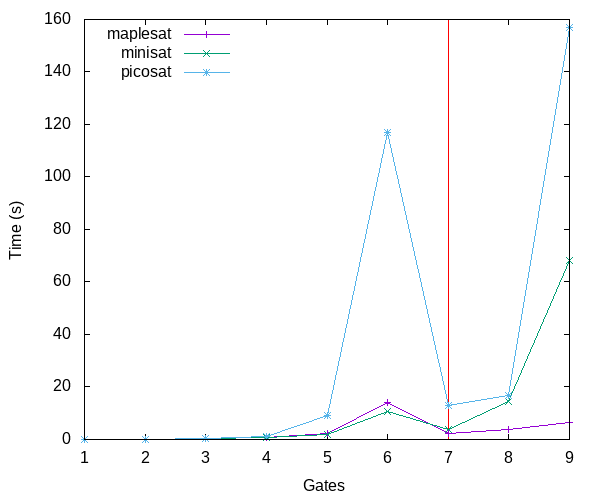
\includegraphics[width=0.8\textwidth]{images/times/8and_kulikov.png}
  \caption{Times taken by SAT solvers to check for existence of a circuit computing AND on 8 bits, using the Kojevnikov reduction\label{fig:8and_kulikov}}
\end{figure}

\clearpage

\begin{figure}[h!]
  \centering
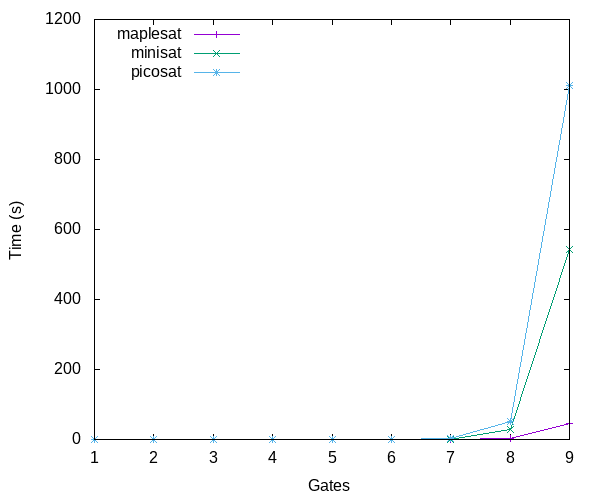
\includegraphics[width=0.8\textwidth]{images/times/4parity_naive.png}
\caption{Times taken by SAT solvers to check for existence of a circuit computing parity on 4 bits, using the Naive reduction\label{fig:4parity_naive}}
\end{figure}

\subsection{Comparison of SAT solvers and reductions} \label{satresults}

We were interested in what would be the fastest solver and reduction to use for further experiments, so we investigated whether there was a relationship between the reduction used to encode a Boolean function, the solver used, and the time taken by the solver. We are not aware of any prior investigation into this area.

We used the same three reductions and the MiniSAT, PicoSAT, and MapleSAT solvers. Glucose-Syrup was not included since it is a parallel solver, meaning the amount of time it takes is subject to different factors, e.g. number of threads available from the hardware and parallelisability of the problem, so it is not comparable.

We took the total of the times each combination took to solve the problems from Section \ref{funcresults} and compared them as shown in Figure \ref{fig:totals}. It can be seen that MapleSAT on the Kojevnikov encoding performs the best. Apart from this, the effect of the reduction and the solver seem to be independent.

\begin{figure}[h!]
  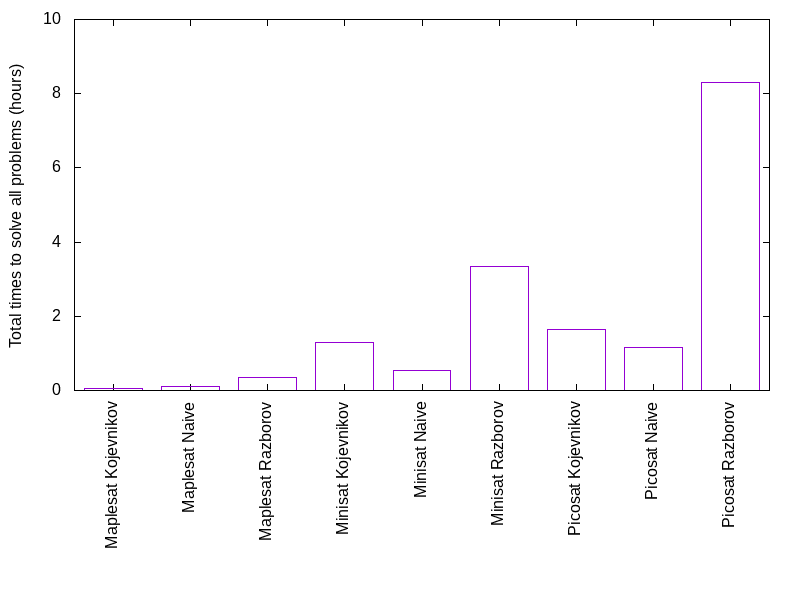
\includegraphics[width=\textwidth]{images/totals.png}
  \caption{Comparison of times taken by SAT solvers on different reductions}
  \label{fig:totals}
\end{figure}

MapleSAT consistently performs better than MiniSAT and PicoSAT (probably because it is the most recent and builds upon the research that went into the other two), and PicoSAT sometimes `spikes' far more badly on difficult problems than the other two, suggesting something about its modifications makes it especially unsuited for solving these reductions.

The Naive and Kojevnikov reductions both performed better than the Razborov reduction, but which was best depended on the solver used. It is possible that the efficient encoding of the Razborov reduction is detrimental to the performance of the solver. However, these results are only applicable to small values of n; possibly at large sizes the efficient encoding would lead to a noticeably smaller search space and make the problem easier to solve.

\subsection{Extension axioms}\label{extresults}

We investigated the effect of adding 50,000, 100,000, and 200,000 extension variables to the encodings for existence of 9-gate circuits for 4-bit \(MOD_3\) and 4-bit parity functions. The literals were chosen uniformly at random using a pseudorandom number generator simulating a uniform distribution (specifically, xorshift128+ due to the TypeScript implementation). Taking note of the results from the previous section, we used the Kojevnikov reduction and MapleSAT.

The results are displayed in Figures \ref{fig:extparity} and \ref{fig:extmod3} as boxplots, where each `box' contains half of the datapoints for that result, and the median is shown as a horizontal line dividing the box in half. The lines above and below each box (`whiskers') show the maximum and minimum, with all datapoints lying between them.

On the \(MOD_3\) function, adding extension variables consistently increased the time for the solver, possibly due to a larger amount of clauses and variables needing to be dealt with at each step. However, for the parity function, adding 100,000 and 200,000 variables led to a speedup over 50 percent of the time. For both functions the median time was lowest when adding 100,000 variables, suggesting that this is a proportionate amount for the size of the problem (both problems had 401 variables and 37500 clauses, although a few of these were single-literal clauses that can be immediately simplified away by the solver).

\begin{figure}[h!]
  \centering
  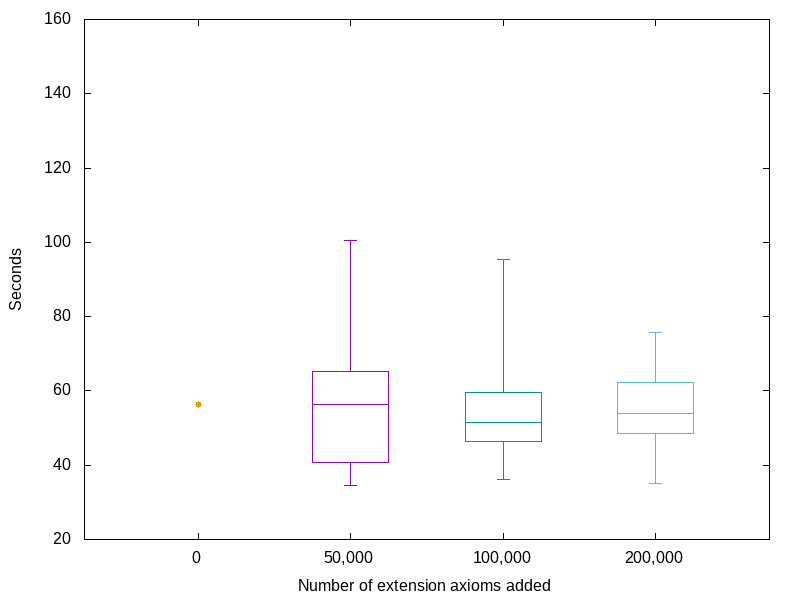
\includegraphics[width=0.8\textwidth]{images/extvars/boxplot_4parity_medians.png}
  \caption{Comparison of times taken to check existence of a 9-gate circuit for 4-bit parity  \label{fig:extparity}}
\end{figure}

\clearpage 

  \begin{figure}[h!]
  \centering
  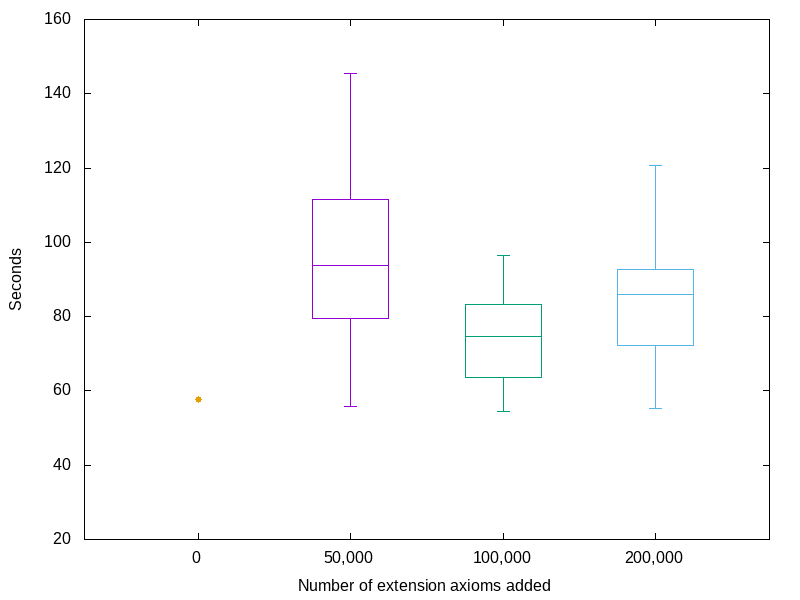
\includegraphics[width=0.8\textwidth]{images/extvars/boxplot_4mod3_medians.png}
  \caption{Comparison of times taken to check existence of a 9-gate circuit for \(MOD_3\)  \label{fig:extmod3}}
\end{figure}


\subsection{Random functions}\label{randomresults}

After seeing the variation in times between functions in the previous sections, we decided to investigate the overall distribution of times for functions with the same input size. We decided to investigate 4-bit functions, as Knuth did in ~\cite{knuth15} (Section 7.1.2, Table 1) but for the De Morgan basis rather than the full basis. However, while he checked all 65536 functions, we chose to take a random sample of 64 functions rather than checking all of them. This has the advantage that the experiment could be completed in a small amount of time even for larger input sizes, where checking all functions would be infeasible due to the difficulty of the problems and the large number of functions. 

64 truth tables were generated for 4-bit inputs, uniformly setting the output bit to 0 or 1 for each input, using the same pseudorandom generator as above. The existence of circuits of size 1 to 11 for these tables were encoded with the Kojevnikov reduction and solved using MapleSAT. 

The times taken to check for circuits are shown plotted against their optimal circuit size in \ref{fig:4rand_scatter} (note that 2 tables could not be fully solved within 9 hours; these functions have been omitted leading to a sample size of 62). The distribution of optimal circuit sizes is shown in \ref{fig:4rand_sizes}.

\begin{figure}[!h]
  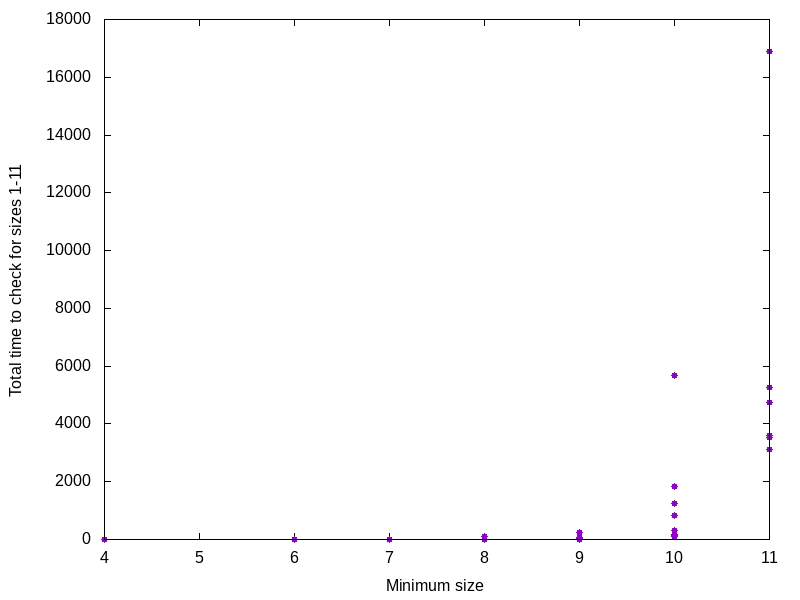
\includegraphics[width=\textwidth]{images/random/4bit_scatter.png}
  \caption{Time taken to check up to 11 gates for randomly chosen functions}
  \label{fig:4rand_scatter}
\end{figure}

The scatter graph shows a clustering in times between functions of the same optimal circuit size, but with a few outliers taking more time. This is most easily seen for sizes 10 and 11 (although the same is visible for 8 and 9 when plotted on a smaller scale). Also, the clustered functions of each optimal circuit size took strictly less time to solve than those with larger sizes, despite the fact that we always checked for existence up to 11 gates. On closer inspection of the times for each function, a spike in length on or around the minimum size was usually observed, similarly to in \ref{satresults}. This shows a generally strong relationship between the difficulty of checking circuit existence and the complexity of the function.

\begin{figure}[!h]
  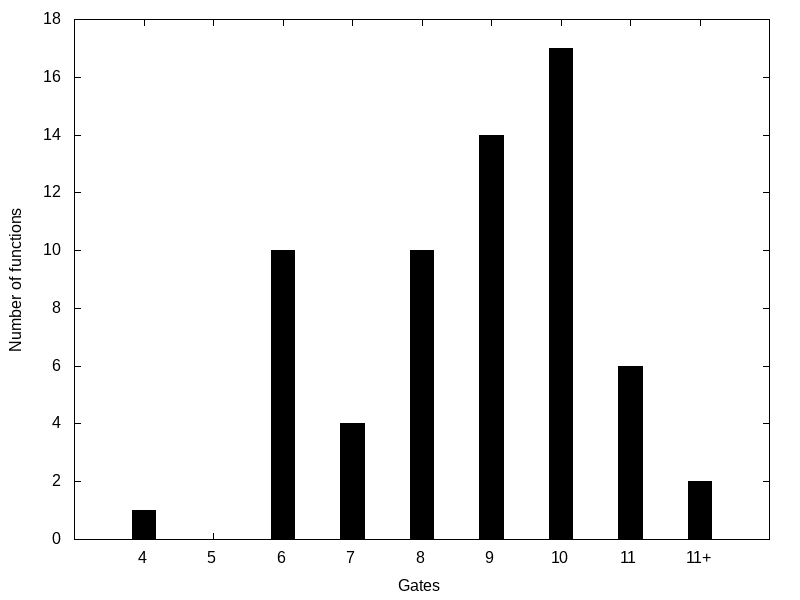
\includegraphics[width=\textwidth]{images/random/4bit_sizes.png}
  \caption{Sizes of optimal circuits for 4-bit functions with randomly chosen truth tables}
  \label{fig:4rand_sizes}
\end{figure}

While we expect a large proportion of circuits to be hard (i.e. have a large optimal circuit size) for large input sizes ~\cite{arora}, the usual counting arguments break down for such small values of n due to large coefficients for the circuit encoding size. However, using the SAT solver we can check the number of hard circuits directly. While the small sample size can account for the irregular shape of the graph in \ref{fig:4rand_sizes}, there does appear to be a peak around 10 gates. This contradicts the intuition that there should be exponentially more harder functions, and suggests that there is quite a low upper limit on the complexity of a function which only can only vary over 4 bits of input. 

While this is all under the assumption that the pseudorandom generator used did output a truly random sample (in reality, it may have sampled disproportionately many easy or hard functions), it is encouraging that Knuth's results for all functions in~\cite{knuth15} also follow a curve similar to ours - although since his basis was $B_2$, where gates can compute more complex functions, the maximum size of any circuit was only 7 and the size with the most functions was 5. This suggests that our method could still provide a good approximation of the space of all functions, even for bigger input sizes.

\begin{figure}[!h]

  \begin{minipage}{0.45\textwidth}
  \begin{centering}
  \begin{tabular}{ |c|c| }
  \hline
  Input & Output \\ 
  \hline
  0000 & 1 \\
  0001 & 1 \\
  0010 & 1 \\
  0011 & 0 \\
  0100 & 0 \\
  0101 & 1 \\
  0110 & 0 \\
  0111 & 0 \\
  1000 & 0 \\
  1001 & 1 \\
  1010 & 1 \\
  1011 & 0 \\
  1100 & 1 \\
  1101 & 0 \\
  1110 & 1 \\
  1111 & 1 \\
  \hline
  \end{tabular}
  \end{centering}
  \caption{Example truth table for function with optimal size 11 that took 87 minutes to solve all sizes}

  \

  \begin{centering}
    \begin{tabular}{ |c|c| }
    \hline
    Input & Output \\ 
    \hline
    0000 & 0 \\
    0001 & 0 \\
    0010 & 1 \\
    0011 & 0 \\
    0100 & 0 \\
    0101 & 1 \\
    0110 & 1 \\
    0111 & 0 \\
    1000 & 1 \\
    1001 & 1 \\
    1010 & 0 \\
    1011 & 1 \\
    1100 & 0 \\
    1101 & 0 \\
    1110 & 0 \\
    1111 & 0 \\
    \hline
    \end{tabular}
    \end{centering}
    \caption{Example truth table for function with optimal size 10 that took 95 minutes to solve all sizes}

\end{minipage}\hfill
\begin{minipage}{0.45\textwidth}
  \begin{centering}
    \begin{tabular}{ |c|c| }
    \hline
    Input & Output \\ 
    \hline
    0000 & 1 \\
    0001 & 1 \\
    0010 & 0 \\
    0011 & 1 \\
    0100 & 0 \\
    0101 & 1 \\
    0110 & 1 \\
    0111 & 1 \\
    1000 & 0 \\
    1001 & 0 \\
    1010 & 1 \\
    1011 & 0 \\
    1100 & 1 \\
    1101 & 1 \\
    1110 & 1 \\
    1111 & 0 \\ 
    \hline
    \end{tabular}
    \end{centering}
    \caption{Example truth table for function with optimal size 11 that took 282 minutes to solve all sizes}

    \
    
    \begin{centering}
      \begin{tabular}{ |c|c| }
      \hline
      Input & Output \\ 
      \hline
      0000 & 0 \\
      0001 & 1 \\
      0010 & 0 \\
      0011 & 0 \\
      0100 & 0 \\
      0101 & 0 \\
      0110 & 0 \\
      0111 & 1 \\
      1000 & 0 \\
      1001 & 0 \\
      1010 & 0 \\
      1011 & 1 \\
      1100 & 1 \\
      1101 & 1 \\
      1110 & 1 \\
      1111 & 0 \\
      \hline
      \end{tabular}
      \end{centering}
      \caption{Example truth table for function with optimal size 10 that took 31 minutes to solve all sizes}
  \end{minipage}
\end{figure}

\clearpage

\subsection{Knuth's MOD-3 conjecture}\label{knuthresults}

Finally, we decided to check whether the power of SAT solvers and the available computing power had progressed enough from the previously published papers to allow us to solve new problems. For this we decided to re-investigate Knuth's conjecture about the circuit size for modulo 3 functions. 

Since he was able to confirm that for the $B_2$ basis $size(MOD^{m,r}_n) = 3n - 5 - [(n+r) \equiv 0 \ mod \ 3] $ for $3 \leq n \leq 5$ and all $r$, and for the case $n=6, r=0$, but not for the case $n=6, r=1$, we decided to try and check the hypothesis for $n=6, r=0$ and $n=6, r=1$ for the De Morgan basis. This involved checking for circuits for the function up to size 11 and 12, and 12 and 13 respectively. 

The Glucose-Syrup solver was used, running on the Oxford ARC service with a maximum of 32 threads (so, 32 parallel instances of the solver working together). In order to ensure that the number of threads would lead to a gain in performance, rather than a drop due to the extra time needed to coordinate them, the SAT solver was timed on a smaller problem with 4, 8, 16 and 32 threads; it displayed gains in performance up to 32. 

For the De Morgan basis, it was shown that Knuth's conjecture does not hold for $n=6, r=0$; confirming that there is no circuit size 11 took only 17 minutes, but confirming there is none of size 12 took 72.97 hours.

For $n=6, r=1$, confirming that there is no circuit size 12 took 175.37 hours, while checking for size 13 did not terminate within the alloted 2 weeks of runtime, corroborating Kulikov et al's account in~\cite{kulikovlocal} that solvers cannot yet handle circuits of size 13 or higher.

We also attempted to check $n=6, r=1$ for the $B_2$ basis, but again the solver did not terminate within 2 weeks.

\section{Discussion}

\subsection{Reflection}

The main practical lesson learned from this project was to think in the long term. Firstly, by writing code that can easily be adapted, i.e. following good OOP practices, so that less refactoring will be needed later, and by writing code that can scale to dealing with larger numbers as the scope and ambition of the project expands. This could be done by choosing a well-suited programming language, algorithms and data structures - I chose TypeScript (a statically typed variant of Javascript) and used arrays to store my CNF formulae, since these were familiar and easy for me to get started with, but the performance of my code on large circuits was an unexpected barrier later on, as well as the poor documentation of the different pseudorandom generators in TypeScript. Also, I was often too focused on quickly getting results rather than investing time in creating a convenient interface for the experiments or processing the resulting data, which led to wasted time in the long run.

On the academic side, I have begun to learn how to read and extract the information I need from papers, as well as how to write in the academic style and include a sufficient amount of references and background for my own report. I discovered that doing academic research is like any creative creative process, involving exploration, creativity, backtracking and the need to unify the ideas of the project into a central narrative. Furthermore, clear communication and precision is important, something I found out when I wrongly assumed the definitions of some common Boolean functions. I practiced analysing data, looking for patterns, applying my theoretical knowledge and drawing conclusions about the things that I was investigating. I also learned some techniques for visualising data in order to highlight the patterns within it to the reader.

I have begun to get a feel for how SAT solvers can be used in theoretical Computer Science. I have observed some of the current capabilities of solvers, the categories under which they are judged (such as general, industrial, and parallel) and the algorithms which power them, including by coding my own basic DPLL algorithm during preliminary experiments. I have learned more about the current state of research in circuit complexity and learned the idea of proof complexity as a result of my background reading, as well as discovering the various barriers that actually make proving the P vs NP problem so difficult.

The timeline of my work on the project began with writing a Javascript program to reduce a single circuit to SAT using the Kojevnikov reduction. I quickly found it unwieldy and wrote a library of TypeScript objects to make it easy to read truth tables from files, store CNFs, quickly add certain types of clauses to them, and output them in the DIMACS format used by the SAT solvers. 

Next I wrote reductions to various types of restricted circuits, such as monotonic, bounded-depth, and unbounded fan-in. However, since the problems for restricted circuits did not seem to be consistently harder or easier to solve in my preliminary experiments, I decided to focus on improving the performance for general circuits.

I read about the Razborov reduction and wrote the program for it, as well as for the naive reduction. I investigated the different reductions' performances with the three SAT solvers at this point, in order to select the fastest one for use in further experiments, and concluded that I should use the Kojevnikov reduction with the MapleSAT solver.

Realising that more precise measurements were needed for the experiments, I investigated better methods to record the runtime of programs on the command line, beginning with using the `time' command but progressing to storing the local start and end time in shell variables for greater accuracy, and outputting the time elapsed to text files together with additional columns of data to make it easier to understand and plot. I also gained a greater proficiency in using stream editors and gnuplot on the command line in order to process the data from my experiments, and learned \LaTeX  \ in order to present the results and theory necessary for my report.

The rest of the project proceeded smoothly, conducting experiments for extension axioms and randomly generated functions, as well as learning how to use the Oxford ARC service with a parallel solver to investigate Knuth's conjecture. 

\subsection{Conclusions}

We have confirmed that when conducting empirical investigation of circuit lower bounds, both the SAT solver and the SAT reduction used are critical for getting results without using too much time and resources, and the effect that each has is not always independent. This is an area that prior work in the field had neglected. We demonstrated some different uses of the SAT solver to investigate theoretical ideas, including how high-powered computing can be incorporated to check for bigger circuits. 

We also discovered that the amount of time it takes to check circuit existence for a function is related to the minimum size of its circuit, and that it usually takes longer when checking for a size that is closer to the minimum, although larger sizes are also usually more difficult. This suggests that there may be other ways to investigate, such as guessing the minimum size and checking on either side of it, or checking in parallel, rather than doing a linear search.

\subsection{Further directions}

Building on the experiments so far, it seems feasible to search for the circuit size for all 4-bit functions, as Knuth did, in order to understand the distribution of minimum sizes for small inputs and see if it differs significantly in the $U_2$ basis. Our sampling method could also be used to investigate bigger inputs, where checking all functions would be infeasible due to the sheer number, such as 9-bit inputs. For these input sizes, the counting argument proof that most circuits are exponential would apply, and we would be able to verify this experimentally. Circuits with restricted depth, different bases and higher fan-in could also be investigated, for example to verify some of the stronger lower bounds that have been proved for them.

The fact that extension axioms leading to improvements were found, even with no strategy or constraints on the axioms added, is promising for research in the topic. Even without theoretical research into strategies for adding the extension axioms, it would be interesting to do data analysis on a larger sample of randomly generated extension variables - for example, measuring the improvement in performance against the depth of circuits added, or whether literals are chosen from the variables determining gate types or those determining graph edges.

It would also be a good idea to compare how more recent SAT solvers do on the MCSP, analyse the reasons behind the better performance of certain ones using prior research into SAT solvers, and explore how they might be customised to suit the problem better. Similarly, it would be interesting to compare the Kojevnikov reduction to even more types of reductions and analyse why SAT solvers perform better on some than others.

\bibliographystyle{plain} 
\bibliography{sources}

\section{Appendix}

\subsection{Graphs of solver performance when checking for existence of circuits computing various symmetric functions}

\begin{figure}[h!]
  \centering
  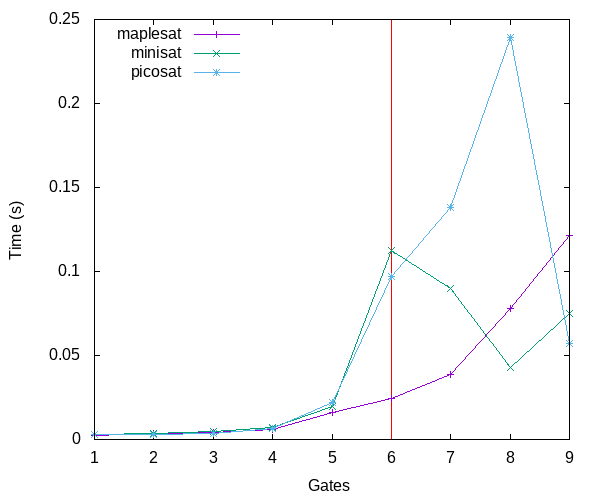
\includegraphics[width=0.8\textwidth]{images/times/3mod3_kulikov.png}  
  \caption{$MOD_3$ on 3 bits, Kojevnikov encoding}
\end{figure}
\begin{figure}[h!]
\centering
  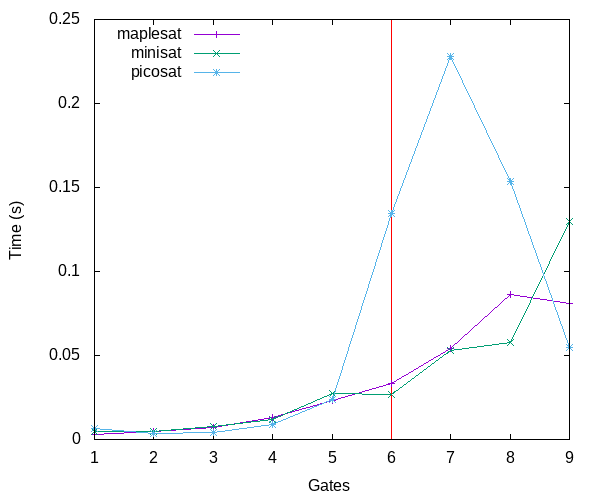
\includegraphics[width=0.8\textwidth]{images/times/3mod3_naive.png}  
  \caption{$MOD_3$ on 3 bits, Naive encoding}
  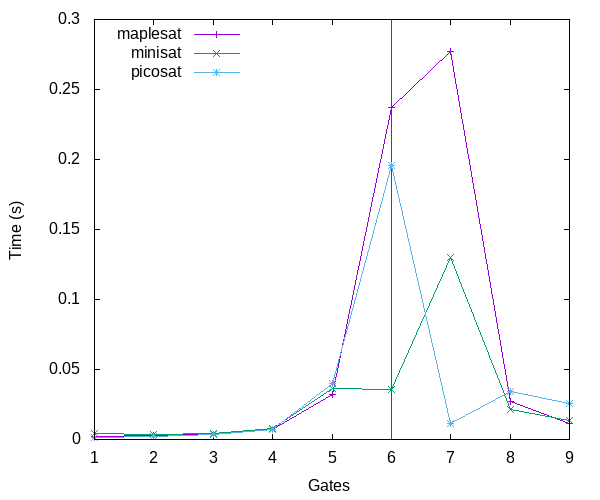
\includegraphics[width=0.8\textwidth]{images/times/3mod3_raz.png}  
  \caption{$MOD_3$ on 3 bits, Razborov encoding}
\end{figure}
\begin{figure}[h!]
\centering

  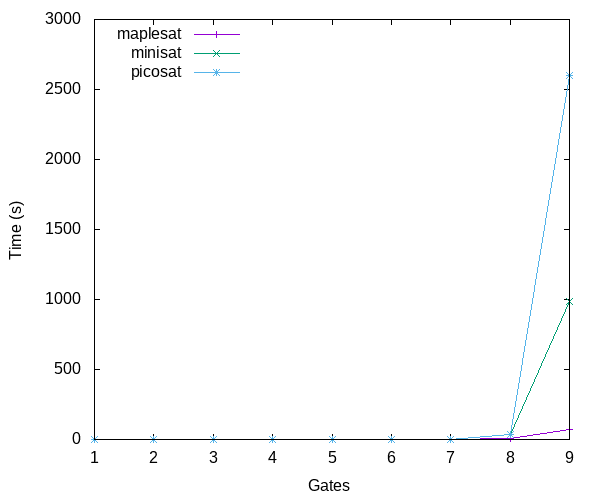
\includegraphics[width=0.8\textwidth]{images/times/4mod3_naive.png}  
  \caption{$MOD_3$ on 4 bits, Kojevnikov encoding}
  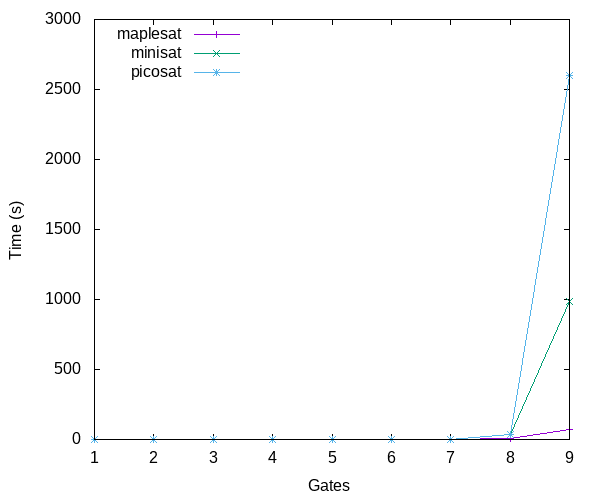
\includegraphics[width=0.8\textwidth]{images/times/4mod3_naive.png}  
  \caption{$MOD_3$ on 4 bits, Naive encoding}
\end{figure}
\begin{figure}[h!]
\centering
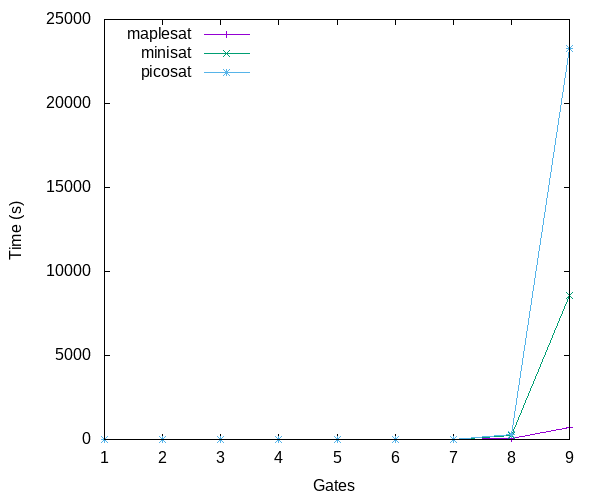
\includegraphics[width=0.8\textwidth]{images/times/4mod3_raz.png}  
\caption{$MOD_3$ on 4 bits, Razborov encoding}
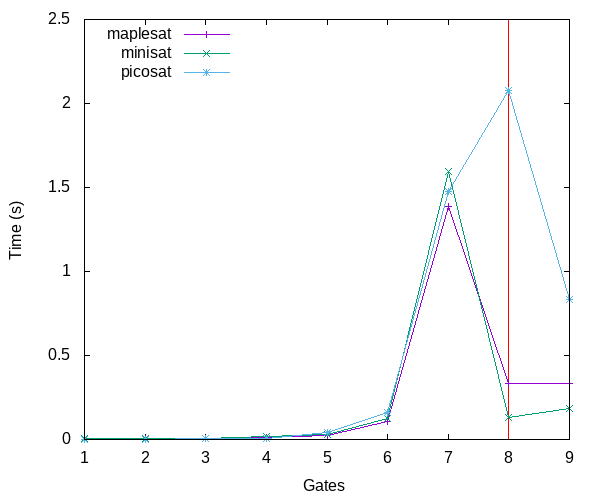
\includegraphics[width=0.8\textwidth]{images/times/3parity_naive.png}  
\caption{Parity on 3 bits, Naive encoding}
\end{figure}
\begin{figure}[h!]
\centering
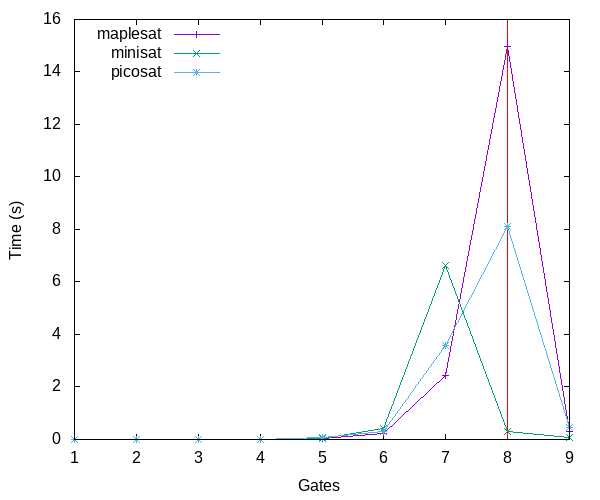
\includegraphics[width=0.8\textwidth]{images/times/3parity_raz.png}  
\caption{Parity on 3 bits, Razborov encoding}
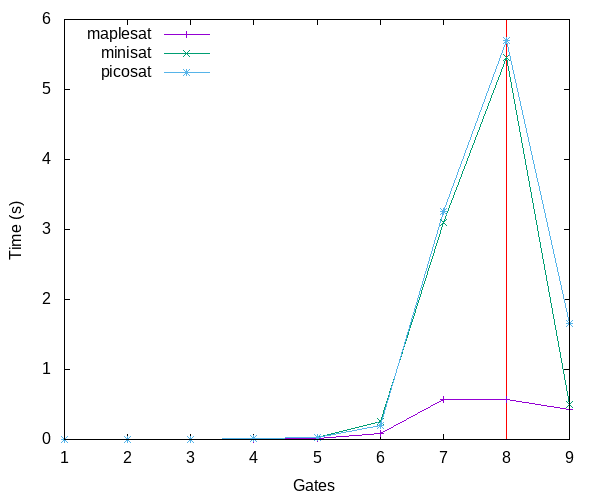
\includegraphics[width=0.8\textwidth]{images/times/3parity_kulikov.png}  
\caption{Parity on 3 bits, Kojevnikov encoding}
\end{figure}
\begin{figure}[h!]
\centering


  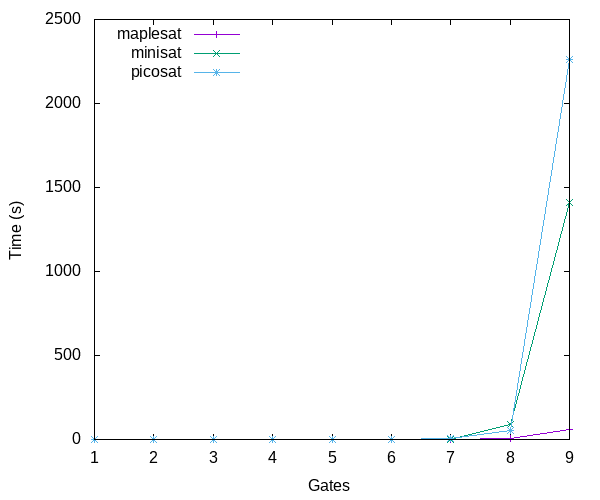
\includegraphics[width=0.8\textwidth]{images/times/4parity_kulikov.png}  
  \caption{Parity on 4 bits, Kojevnikov encoding}
  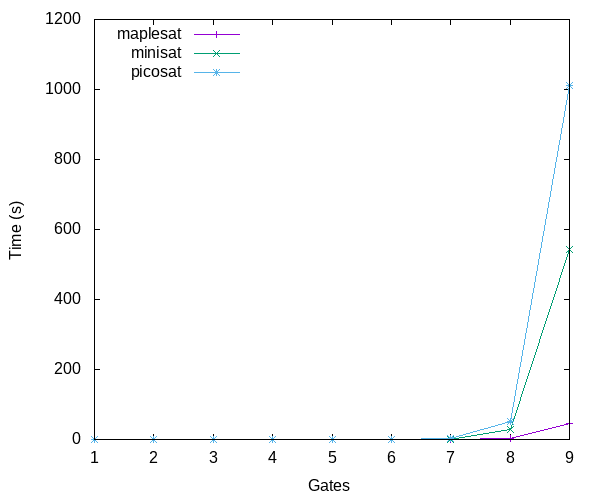
\includegraphics[width=0.8\textwidth]{images/times/4parity_naive.png}  
  \caption{Parity on 4 bits, Naive encoding}
\end{figure}
\begin{figure}[h!]
\centering

  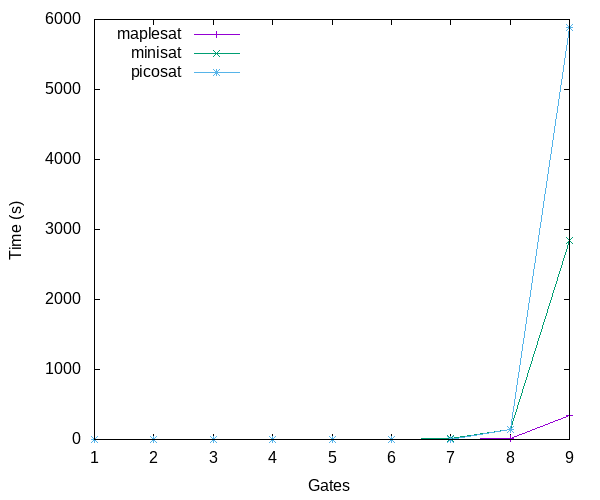
\includegraphics[width=0.8\textwidth]{images/times/4parity_raz.png}  
  \caption{Parity on 4 bits, Razborov encoding}
  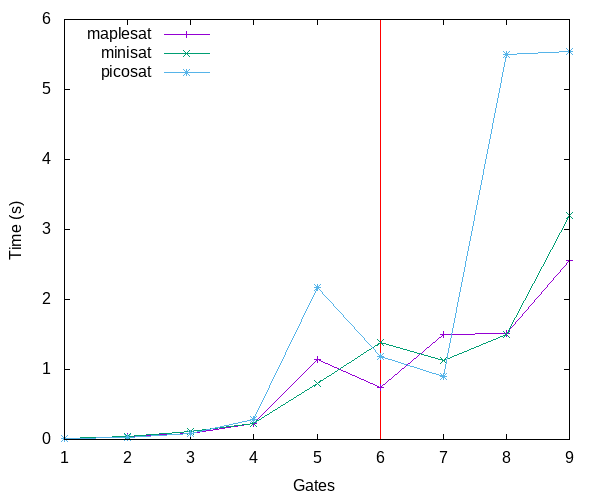
\includegraphics[width=0.8\textwidth]{images/times/7and_kulikov.png}  
  \caption{$AND$ on 7 bits, Kojevnikov encoding}
\end{figure}
\begin{figure}[h!]
\centering

  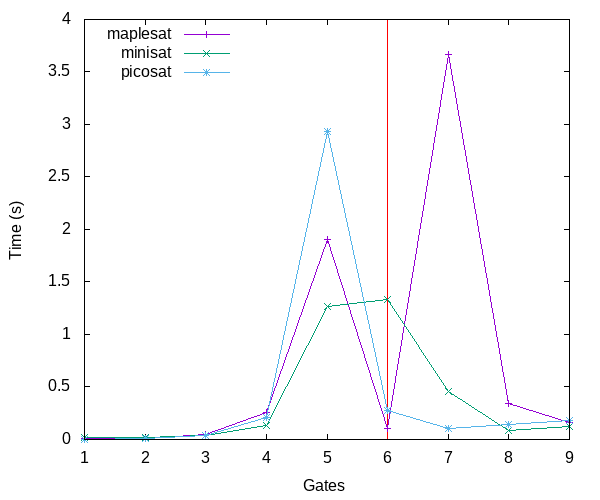
\includegraphics[width=0.8\textwidth]{images/times/7and_naive.png}  
  \caption{$AND$ on 7 bits, Naive encoding}
  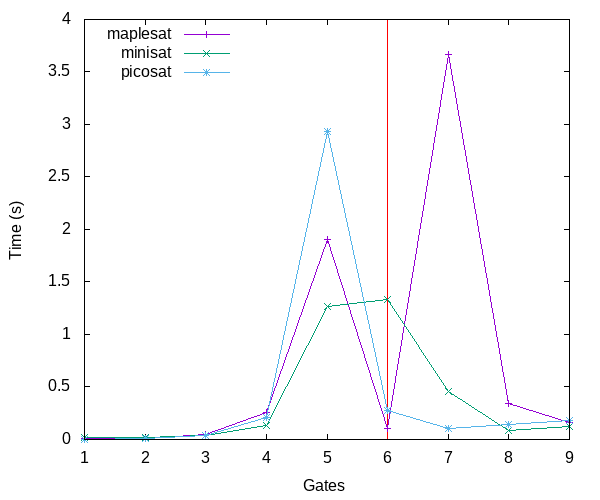
\includegraphics[width=0.8\textwidth]{images/times/7and_raz.png}  
  \caption{$AND$ on 7 bits, Razborov encoding}
\end{figure}
\begin{figure}[h!]
\centering

  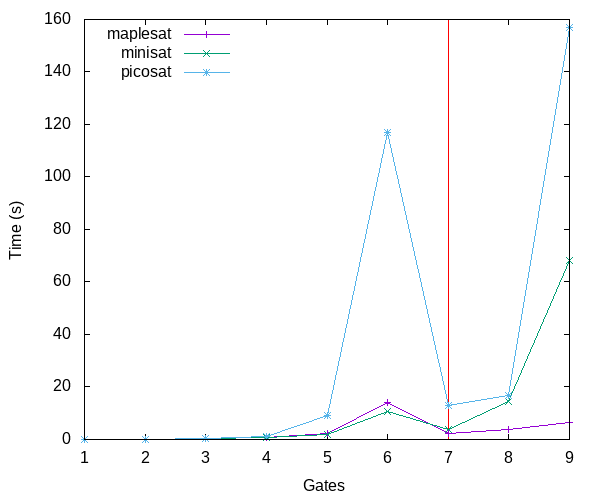
\includegraphics[width=0.8\textwidth]{images/times/8and_kulikov.png}  
  \caption{$AND$ on 8 bits, Kojevnikov encoding}
  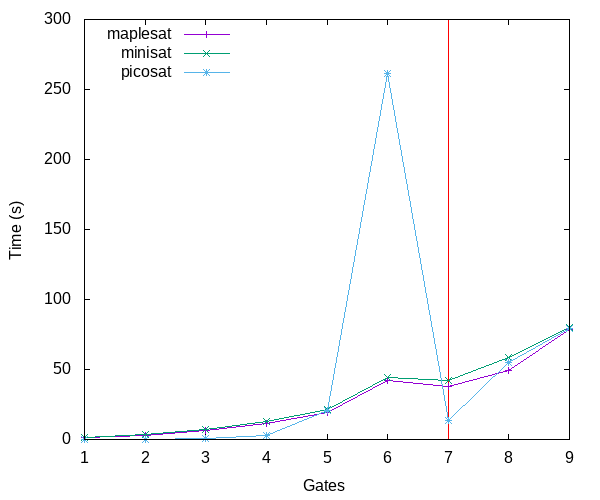
\includegraphics[width=0.8\textwidth]{images/times/8and_naive.png}  
  \caption{$AND$ on 8 bits, Naive encoding}
\end{figure}
\begin{figure}[h!]
\centering

  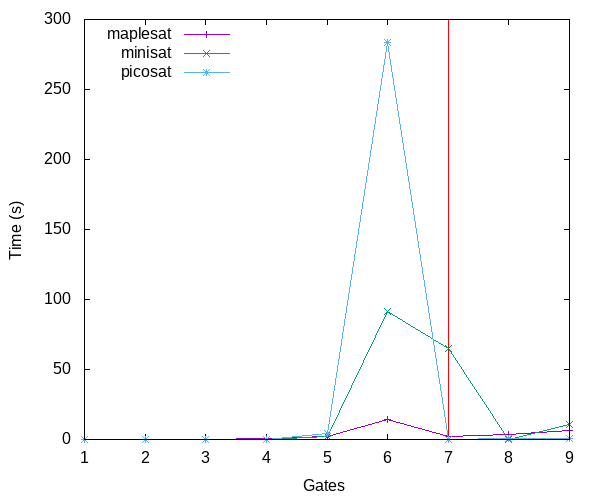
\includegraphics[width=0.8\textwidth]{images/times/8and_raz.png}  
  \caption{$AND$ on 8 bits, Razoborov encoding}
\end{figure}


\end{document}